\mode*

\section{Outline}

\begin{frame}
  \begin{block}{Workshop}
    \begin{itemize}
      \item Outline what's needed to automate reporting to LADOK.
      \item Adapt \texttt{ladok3} and particularly \texttt{weblogin} for MIUN.
      \item Explore how to automate things with Moodle.
    \end{itemize}
  \end{block}
\end{frame}


\section{History}

\begin{frame}
  \vspace{-2cm}
  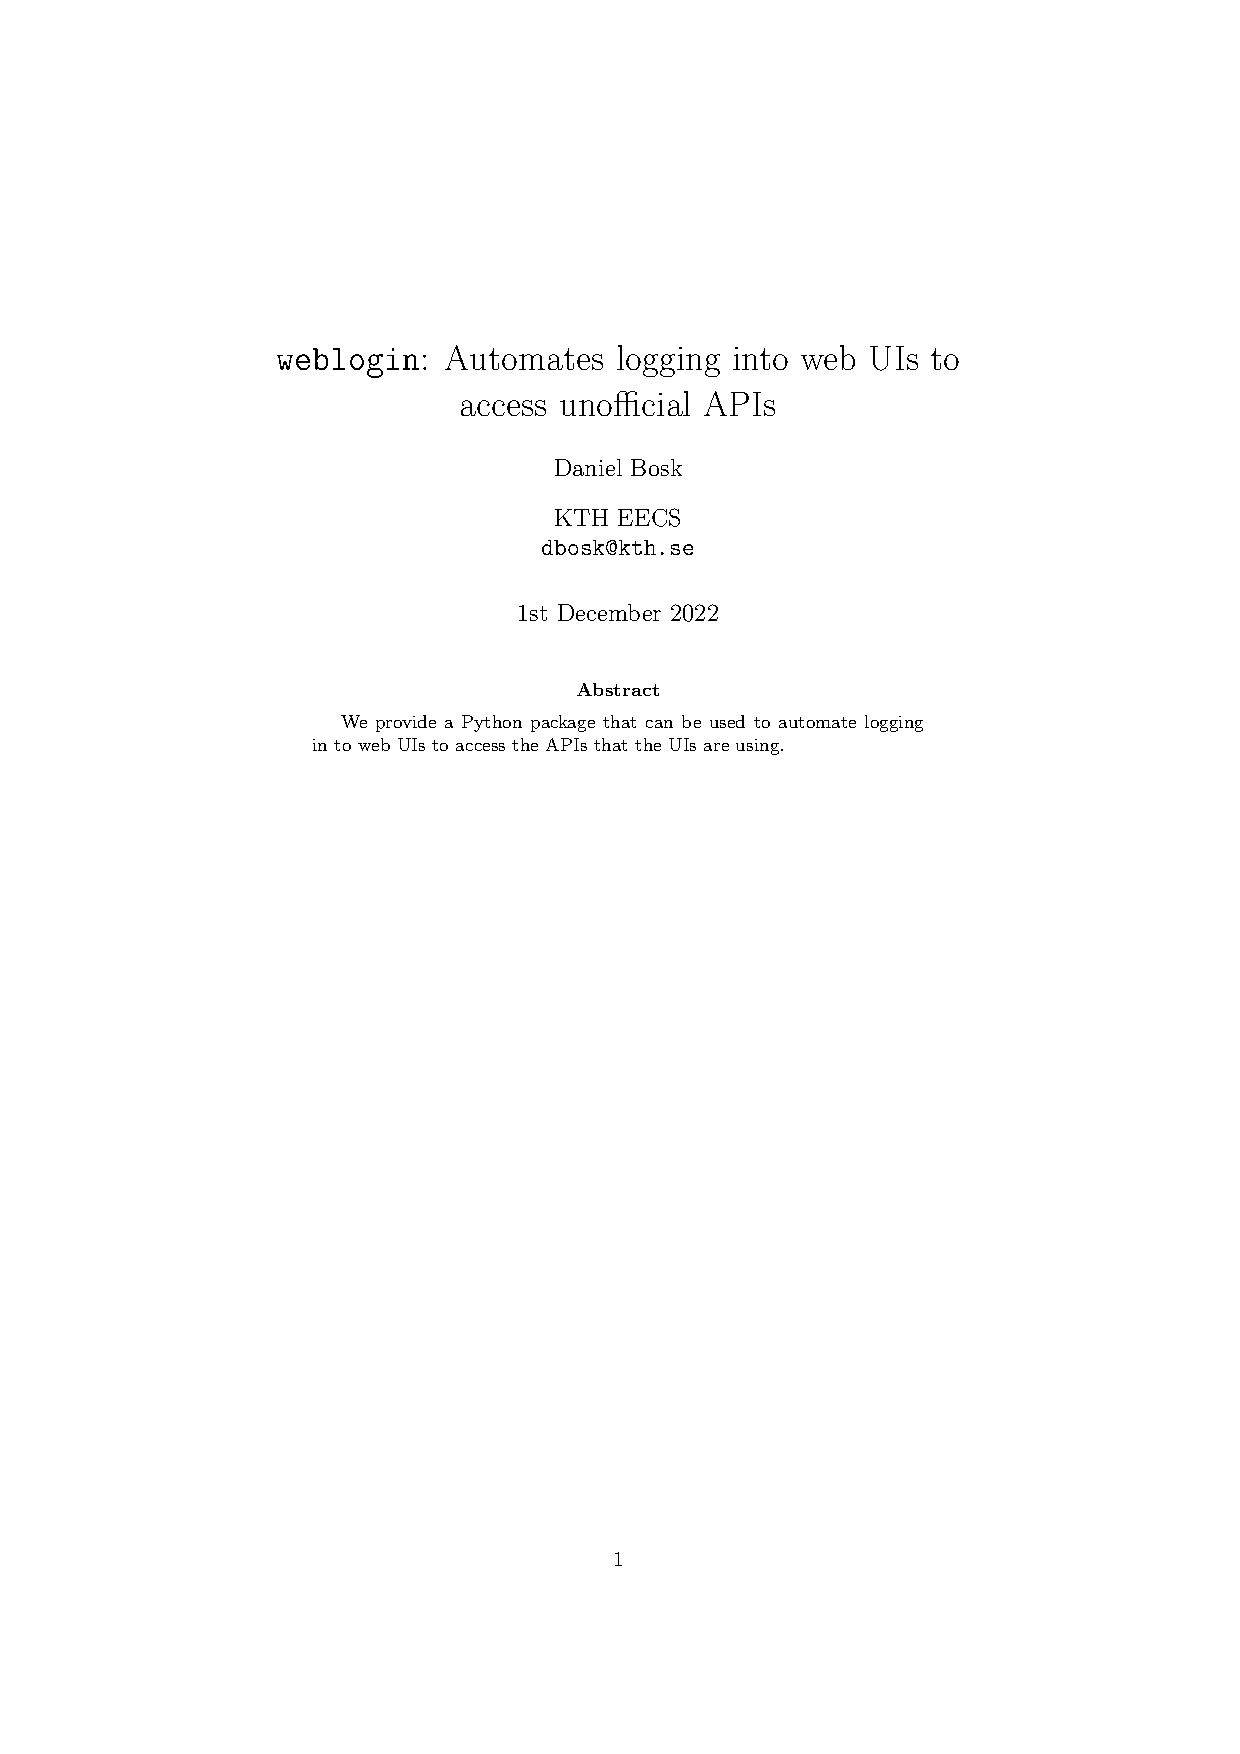
\includegraphics[page=1,width=\textwidth]{figs/weblogin.pdf}
  \vspace{-\textheight}
  \vspace{-2em}
  \begin{question}
    \begin{itemize}
      \item What the **** was that PDF?
    \end{itemize}
  \end{question}
\end{frame}

\begin{frame}
  \vspace{-6.5cm}
  \includegraphics[page=9,width=\textwidth]{figs/weblogin.pdf}
\end{frame}

\begin{frame}
  \begin{block}{Literate programming}
    \begin{itemize}
      \item \fullcite{knuth1984literate}
      \item \textcquote[p.~99]{knuth1984literate}{%
          Let us change our traditional attitude to the construction of 
          programs: Instead of imagining that our main task is to instruct a 
          computer what to do, let us concentrate rather on explaining to human 
          beings what we want a computer to do.%
        }
      \item \url{http://www.literateprogramming.com/}
    \end{itemize}
  \end{block}
\end{frame}


\section{What to do?}

\subsection{Tool development}

\begin{frame}[fragile]
  \begin{block}{Development}
    \begin{itemize}
      \item \url{https://github.com/dbosk/ladok3}
      \item \url{https://github.com/dbosk/weblogin}
      \item \url{https://github.com/dbosk/canvaslms}
    \end{itemize}
  \end{block}

  \begin{block}{Development approach}
    \begin{itemize}
      \item Open source
      \item Independent from institution
    \end{itemize}
  \end{block}
\end{frame}

\subsection{Agenda}

\begin{frame}
  \begin{enumerate}
    \item Look into how to add MIUN/Chalmers login to \texttt{weblogin}.
    \item Look into Moodle's API.
  \end{enumerate}
\end{frame}
